% !TEX root = ../neurosciences-barrels.tex

%%%%%%%%%%%%%%%%%%%%%%%%%%%%%%%%%%%%%%%%%%%%%%%%%%%
%%%%%%%%%%%%%%%%%%%%%%%%%%%%%%%%%%%%%%%%%%%%%%%%%%%
%%%%%%%%%%%%%%%%%%%%%%%%%%%%%%%%%%%%%%%%%%%%%%%%%%%
\section{Introduction}

% \subsection{How to map cortical activity onto the underlying anatomical structure}


The rodent primary somatosensory cortex is a very convenient model for studying the cortical processing of sensory information because of its well defined structural and functional layout that is invariant from animal to animal~\cite{WelkerQuantitative,MeyerCellular,egger_2012}. In its layer IV, neurons are gathered into clusters called barrels that respect the same topology as the whiskers on the snout of the animal~\cite{Woosley-VDLoos}. Each barrel is dedicated primarily to the processing of the input coming from its corresponding whisker (Figure~\ref{somatotopy}A,B).  
When studying sensory processing in the barrel cortex either with electrophysiological or imaging methods, it is therefore of great interest to superimpose the recorded activity onto the underlying barrel topography, which can be reconstructed from the post hoc alignment of tangential brain slices stained for cytochrome oxidase.
In order to optimize this anatomo-functional mapping, which is usually accomplished manually, we developed an automated workflow for the registration of the histological slices of the barrel cortex and the 2-D barrel map reconstruction.


\begin{figure*}[!ht]
\centering
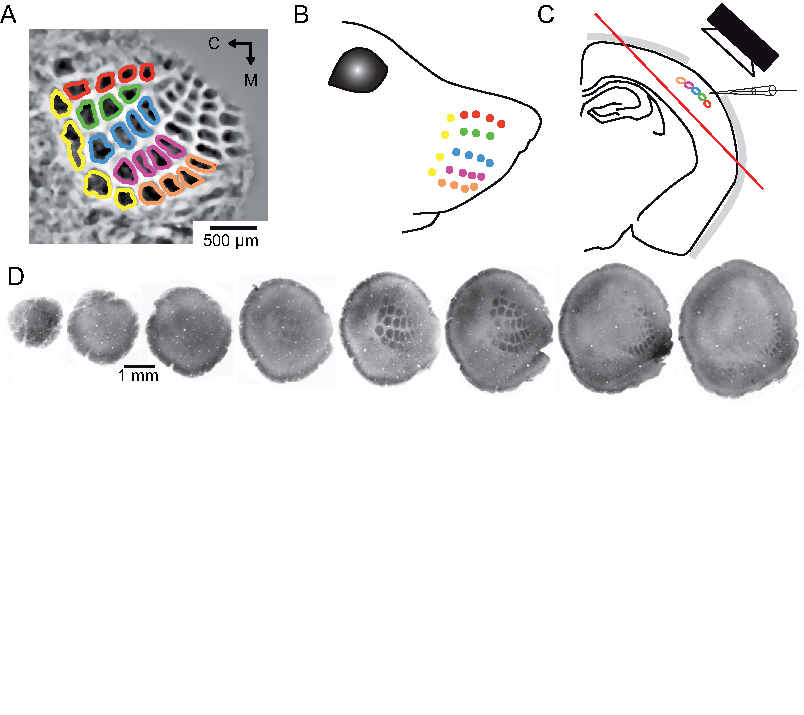
\includegraphics[width=140mm]{images/Perronnet-Figure1}
\caption{
	\textbf{Cytochrome oxidase staining of tangential sections from the mouse primary somatosensory cortex reveals the structural organization of layer 4 barrels that mirrors the arrangement of the vibrissae on 
	the snout.}\\
	%
	\textbf{A.} Following the registration of tangential histological slices and the reconstruction of the barrel map, one can see that the spatial organization of the layer 4 barrels matches the layout of the vibrissae on the snout of the animal (\textbf{B}).  
	%
	\textbf{C.} Drawing of a coronal section of the left hemisphere of the mouse brain illustrating the position of layer 4 barrels within the primary somatosensory area of the cortex. After in vivo imaging of barrel cortex activity, sections are cut tangentially to reconstruct the layer 4 barrel map (cutting plane indicated by the red line).  
	%
	\textbf{D.} A series of tangential histological slices stained for cytochrome oxidase. On the first slice one can see superficial blood vessels. On the other slices, one can see white circular to elliptic spots that correspond to sections of plunging blood vessels. Depending on the exact axis of the cut, barrels can be spread over several slices.
	% 
%	\textbf{C.} Following the registration of tangential histological slices and the reconstruction of the barrel map, one can see that the spatial organization of the layer 4 barrels matches the layout of the vibrissae on the snout of the animal (\textbf{D}). 
}
\label{somatotopy}  
\end{figure*}

Here we focus our attention on voltage sensitive dye imaging (VSDI) of the mouse barrel cortex to illustrate the usefulness of the approach. However, the method can be extended to the study of the rat barrel cortex and applied to other techniques such as 2-photon calcium imaging.  % intracellular or patch-clamp recordings, electrode arrays or 

% Indeed, establishing a precise mapping of the recorded activity onto the underlying cortical cytoarchitecture is highly precious to analyze the cortical processing of sensory perception.

The traditional first step to recover the map of the barrel cortex after imaging experiments is: brain fixation by perfusing the animal with a solution of paraformaldehyde, followed by the cutting of tangential slices ($\sim$100 $\mu$m thick, with or without previous flattening of the cortex), which are subsequently stained for cytochrome oxidase using classical histological procedures that reveal the barrel arrangement in layer IV (Figure~\ref{somatotopy}C,D~\cite{Land-Simons}).

Next, using digital microphotographs of the slices, it is necessary to:
\begin{enumerate}
	\item register the slices ;
	\item fuse the registered slices to define a reconstructed barrel image.
\end{enumerate}
In this article we provide an automated solution for these two steps which are the most time-consuming tasks of the workflow when using conventional manual methods. After completing these steps, it is then relatively simple to define the barrel map by segmenting the reconstructed barrel cortex image. The superimposition of the map with the functional data can be finally achieved by using the superficial blood vessels as anatomical landmarks (Figure~\ref{fig-alignement-superposition}). The proposed anatomo-functional mapping tool significantly speeds up the overall process and provides more accurate anatomo-functional
mapping.


%perform successively the following steps in order to align the barrel map with cortical in vivo recordings:
%\begin{enumerate}
%	\item registration of the slices~;
%	\item fusion of the registered slices to define a reconstructed barrel image~;
%	\item segmentation of the fused image to define the barrel maps~;
%	\item superimposition of the barrel map with the VSDI recording.
%\end{enumerate}
%In this article, we provide an automated solution to the first two steps; this workflow leads to a significant speedup of the overall process and provides more accurate anatomo-functional mapping.



%%%%%%%%%%%%%%%%%%%%%%%%%%%%%%%%%%%%%%%%%%%%%%%%%%%
\subsection{Registration of histological slices}
\label{sec-previous-works}


A typical example of a series of images obtained after the histological process is shown in Figure 1D. Depending on their depth, the histological sections present different properties: in the first section, which corresponds to the surface of the cortex, some large superficial blood vessels are visible together with plunging blood vessels. 
%
This section is crucial for the whole process since it contains most of the superficial blood vessels that will be used for the final alignment of the histological data with the VSDI data (Figure~\ref{fig-alignement-superposition}). The intermediate sections usually contain orthogonal blood vessels (white dots on the slices shown in Figure~\ref{somatotopy}D) that can be used to align subsequent sections. Barrels start appearing on section 3 or 4 and can be visualized on up to 5 sections.

We do not use the deeper sections from subgranular layers as they do not contain any useful information for the reconstruction.



\begin{figure*}[!ht]
\centering
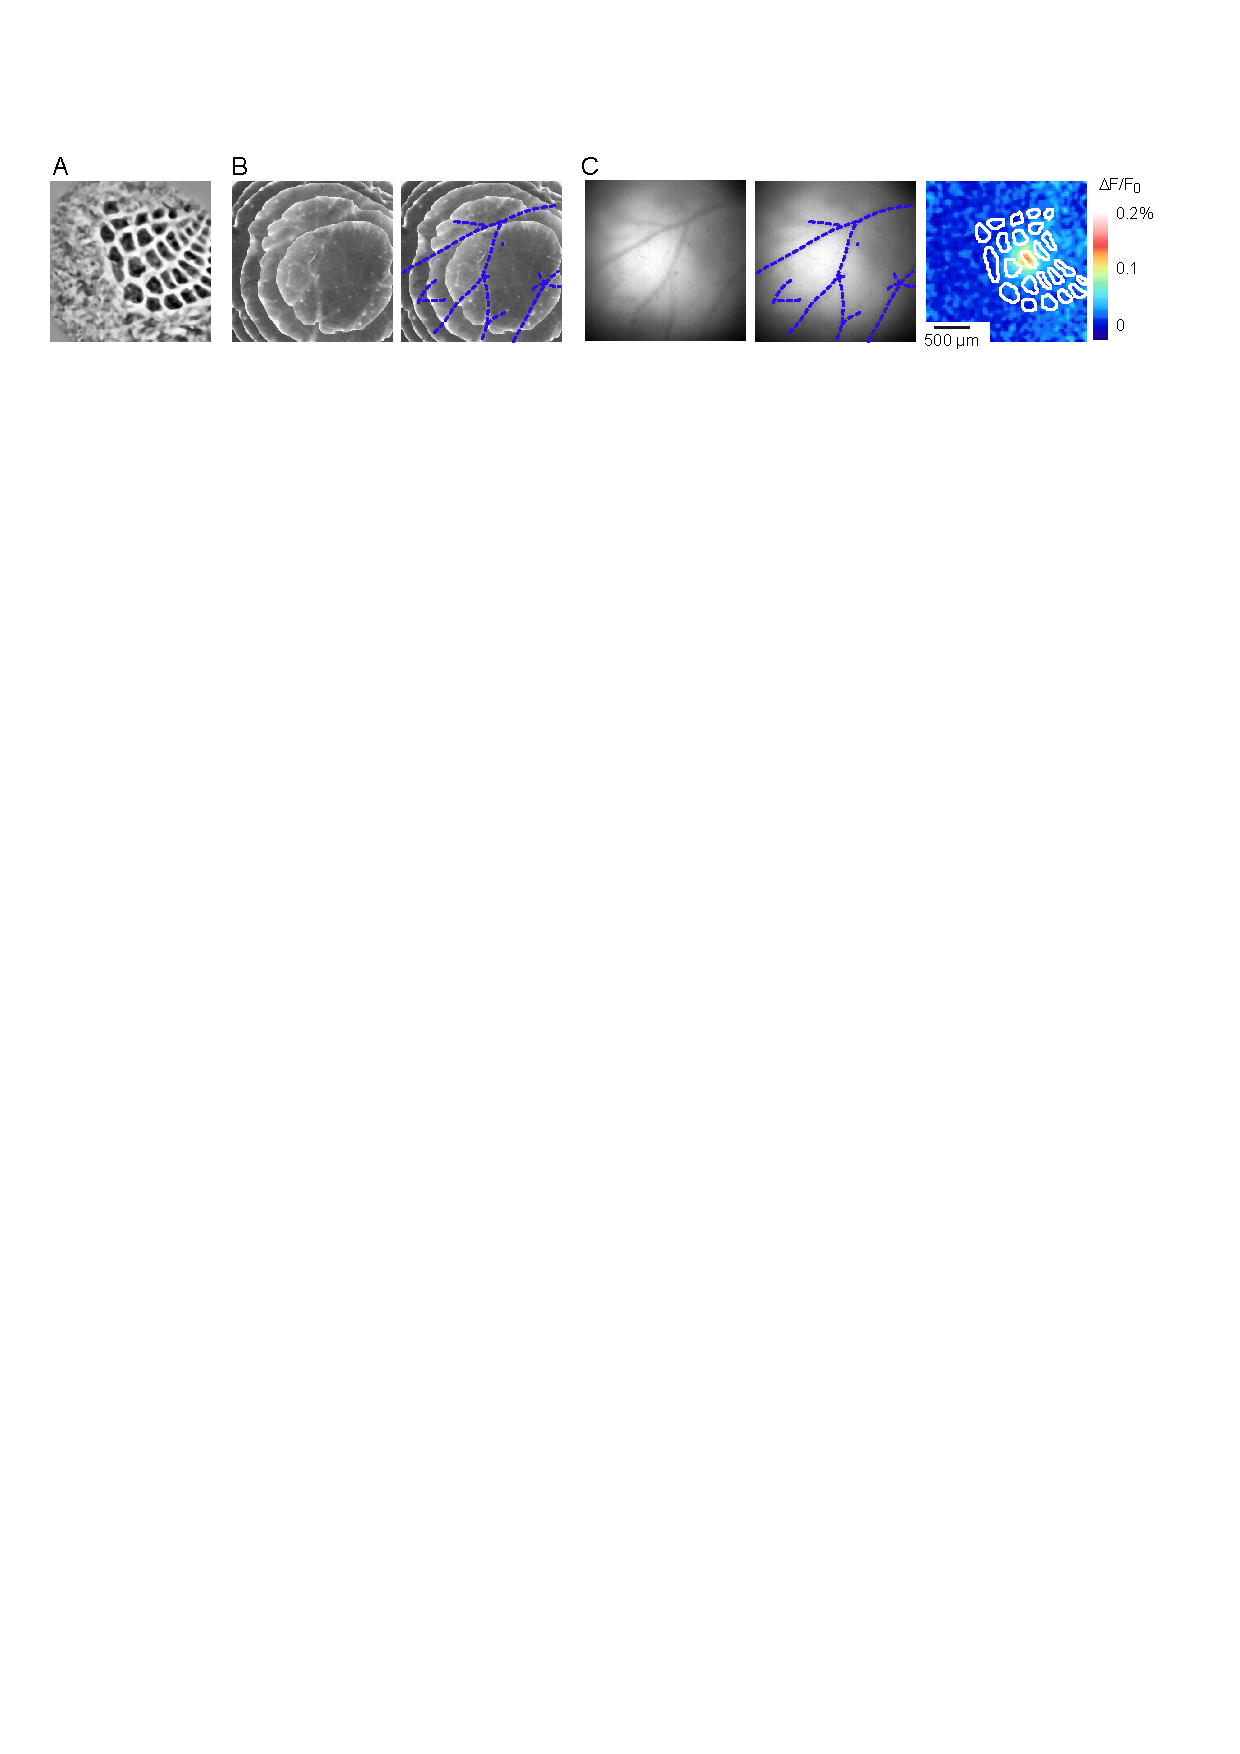
\includegraphics[width=190mm]{images/Perronnet-Figure2}
\caption{
	 \textbf{Alignment of the barrel map with VSDI data using the superficial blood vessels as blueprints.} \\
	 % 
	 \textbf{A.} Barrel map reconstructed from the histological slices shown in figure 1D, using our anatomo-functional mapping method.
	 %
	 \textbf{B.} Superimposition of the registered histological slices, allowing the delineation of the superficial blood vessels (in blue).  
	 %
	 \textbf{C.} The superficial blood vessels also appear in vivo on the fluorescent images taken during the VSDI session. The VSDI data can therefore be aligned with the underlying structural map of the barrel cortex using the blood vessels as anatomical landmarks. On the right, the cortical activity is shown imaged at 10ms following a single C2 whisker deflection with the voltage sensitive dye RH1691 under urethane anesthesia. The barrels outlined from the reconstruction in A are superimposed on the image as white lines.
}
\label{fig-alignement-superposition}  
\end{figure*}



Image registration is a classical problem and its solutions find many applications in medical image analysis. Depending on the imaging modality and the specific prior knowledge of the object to register, a wide variety of methods have been considered in the literature (for an overview see~\cite{GlockerAR,SotirasDP13}). 
%
Only a few previous studies explicitly deal with the problem of registering rodent brain histological sections, usually in order to reconstruct a whole brain in 3D~\cite{ourselin_2001,JuHisto}. 

In order to exploit the microscopic-scale information of the histological data, these applications require the precise registration of a large number of histological slices from the whole brain with a method that accounts for global but also local nonlinear deformations due to tissue shrinkage and tearing after histological preparation. Ourselin et al. presented in~\cite{ourselin_2001} a block matching strategy to compute local similarities and then estimate the rigid transformation that matches the maximum of similar regions in a robust way. Alternatively Ju et al.~\cite{JuHisto} used a method based on pairwise elastic imaging warps, with the specificity to compute the deformation of each section by considering not only two neighbors for each section, but an extended neighborhood including a group of images.

The specific problem of registering histological sections of the rodent barrel cortex has been rarely addressed in the literature. 
%
Egger et al.~\cite{egger_2012} proposed a tool for the 3-D reconstruction and standardization of the rat barrel cortex for the precise registration of single neuron morphology. 
%
Seventy micrometer thick tangential sections of rat barrel cortex are aligned pairwise by finding the rotation and translation that best superimpose blood vessels of two adjacent sections either manually or automatically, using a tool originally developed for the reconstruction of neuronal processes~\cite{DercksenAutomatic}.
% 
Finally the barrels are segmented by using a semi-automated method.
 
% removed
% Note however that the goals and methods of this study~\cite{egger_2012} differ significantly from ours: they rely on a manual segmentation of the barrels, and target a 3-D reconstruction while we focus on a 2-D image fusion using an automated method.

% removed
% In our method, we register the layers by computing a rigid motion to align sets of detected blood vessels (Figure~\ref{fig-algo-sample}A). 

Here we developed a tool to compute the rigid transformations to align sets of detected blood vessels (Figure~\ref{fig-algo-sample}A), and we decided to focus on a 2-D image fusion using an automated method.
%
The usual approach to perform point cloud registration is the iterative closest point (ICP) algorithm introduced by Besl~\cite{besl_1992}. While the initial formulation is not robust to outliers, several approaches explicitly deal with this issue~\cite{chetverikov_2005,nishino_2002,stewart_2002,kaneko_2003,ma_1999}. These approaches are related to re-weighting least squares methods and we propose in~\ref{app-icp} a unifying presentation and convergence analysis of a robust ICP method. 




%%%%%%%%%%%%%%%%%%%%%%%%%%%%%%%%%%%%%%%%%%%%%%%%%%%
\subsection{Fusion of histological slices}

In our framework, the 2-D reconstruction of the barrel maps amounts to perform a fusion of the registered sections (Figure~\ref{fig-algo-sample}B). The goal is to reconstruct the edges of the barrels that are spread over the slices. Image fusion is classically addressed in the field of image processing and computer vision, to perform for instance image editing and stitching. To reconstruct sharp edges, it is necessary to use non-linear methods, the most popular one being based on gradient-domain blending~\cite{perez_2003,raskar_2004}.
%
The goal is to generate a novel image by locally keeping the content of the image having the highest local frequency. In this article, we focus on the use of gradient-domain methods, which have the advantage of being simpler and can be easily tuned for the purpose of barrel map fusion.



%%%%%%%%%%%%%%%%%%%%%%%%%%%%%%%%%%%%%%%%%%%%%%%%%%%
\subsection{Contributions}

Our main contribution is a comprehensive pipeline for the 2-D reconstruction of the barrel cortex from tangential  histological sections. 
% To the best of our knowledge, it is the first time that such a comprehensive framework is developed. 
This pipeline is composed of 2 successive modules that respectively perform: histological section registration and barrel image reconstruction using image fusion. 
%
As a side contribution, we propose to recast the registration problem using a robust ICP optimization method, and we show that a Majorize-Minimize framework can be applied to provably ensure the convergence of the method. 
%
These contributions originate from specific needs raised by studies of sensory integration in the barrel cortex, however the histological section registration tool proposed here might be helpful to reconstruct any anatomical tissue in which blood vessels penetrate predominantly orthogonally to the cutting plane of the histological slices.

